\documentclass[10pt]{beamer}


\usepackage[utf8]{inputenc}
\usetheme{metropolis}
\usepackage{appendixnumberbeamer}
\usepackage{pgfgantt}


\usepackage{booktabs}
\usepackage[scale=2]{ccicons}

\usepackage{pgfplots}
\usepgfplotslibrary{dateplot}

\usepackage{xspace}
\newcommand{\themename}{\textbf{\textsc{metropolis}}\xspace}

\usepackage{array}


\title{High Level Assembler Plugin}
\subtitle{}
\date{Supervisor: Miroslav Kratochvíl}
\author{Michal Bali, Marcel Hruška, Peter Polák, Adam Šmelko, Lucia Tódová}
% \institute{Center for modern beamer themes}
% \titlegraphic{\hfill\includegraphics[height=1.5cm]{logo.pdf}}

\begin{document}

\maketitle


\begin{frame}[fragile]{Motivation}
\centering
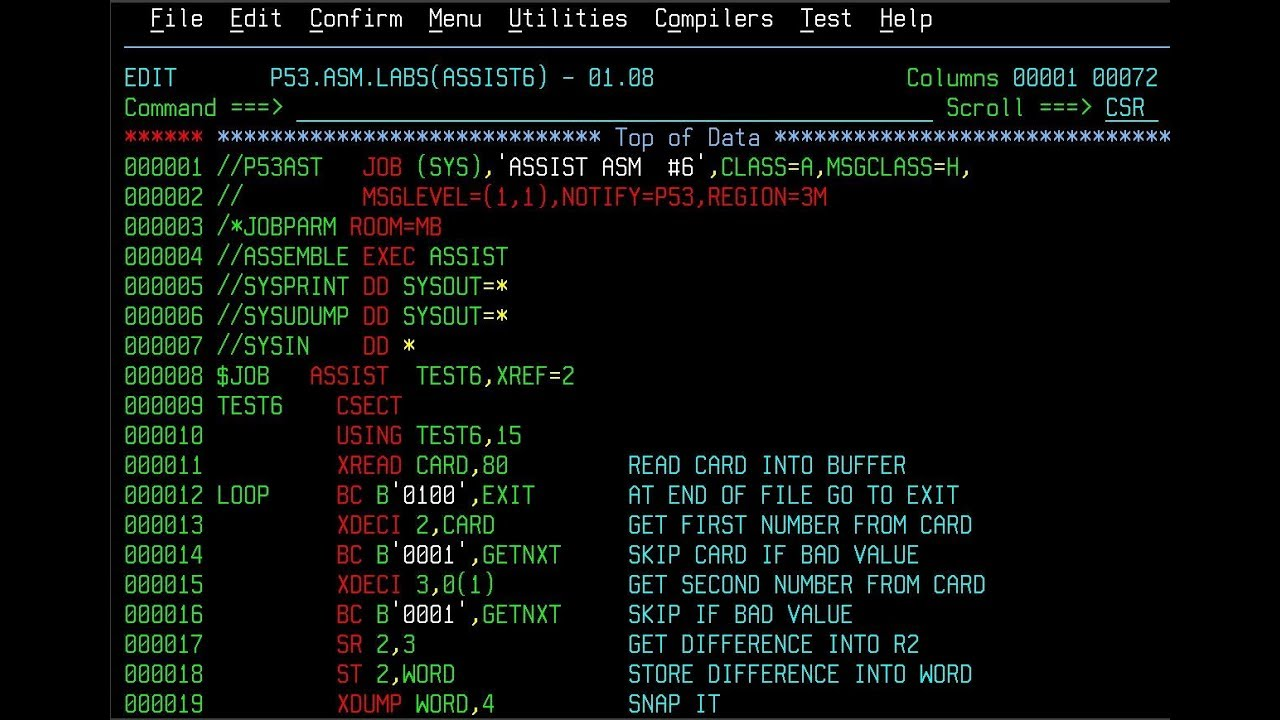
\includegraphics[width=10cm]{img/maxresdefault}

\end{frame}

\begin{frame}[fragile]{Introduction}

    \begin{itemize}
    	\item The aim of the software project is to create an extension that adds language support for HLASM to Visual Studio Code.
    	\item Code validation
    	\item Code navigation (Go to definition, Find all references)
    	\item Tooltips when hovering over symbols
    \end{itemize}
\end{frame}



\begin{frame}[fragile]{The HLASM language}

There are 3 types of instructions:
\begin{enumerate}
	\item Machine instructions
	\item Assembler instructions
	\item Conditional assembly instructions
\end{enumerate}


*Short slide just to introduce instructions*

\end{frame}


\begin{frame}[fragile]{Ordinary assembly example}
  
	\begin{verbatim}
	[00]              LR    1,2
	[01]              DS    CL(LEN)
	[02]   ADDR       DS    CL(SIZE)
	[03]   HERE       DS    CL5
	[04]
	[05]   LEN        EQU   HERE-ADDR
	[06]   SIZE       EQU   1
	\end{verbatim}
	
	\begin{table}[]
		\begin{tabular}{llll}
			\hline
			\multicolumn{1}{|p{1cm}|}{\texttt{2}\hspace{5cm}} & \multicolumn{1}{p{1cm}|}{\texttt{LEN}} & \multicolumn{1}{p{1cm}|}{\texttt{SIZE}} & \multicolumn{1}{p{1cm}|}{\texttt{5}}  \\ \hline
			 &   & \multicolumn{1}{l}{\hspace{-10pt}\rotatebox{90}{\texttt{ADDR->} }}  & \multicolumn{1}{l}{\hspace{-10pt}\rotatebox{90}{\texttt{HERE->}}}                       
		\end{tabular}
	\end{table}
	
\end{frame}

\begin{frame}[fragile]{Conditional assembly example}


\begin{verbatim}
	[00]   &VAR       SETA    1
	[01]   .LOOP      ANOP         
	[02]   SYM        DC      (&VAR)C'A'
	[03]              AIF     (L'SYM GE 10).END
	[04]              MAC     &VAR
	[06]   &VAR       SETA    &VAR+1
	[07]              AIF     (&VAR LE 5).LOOP
	[08]   .END       END     
\end{verbatim}


\end{frame}

\begin{frame}[fragile]{Architecture}
\centering
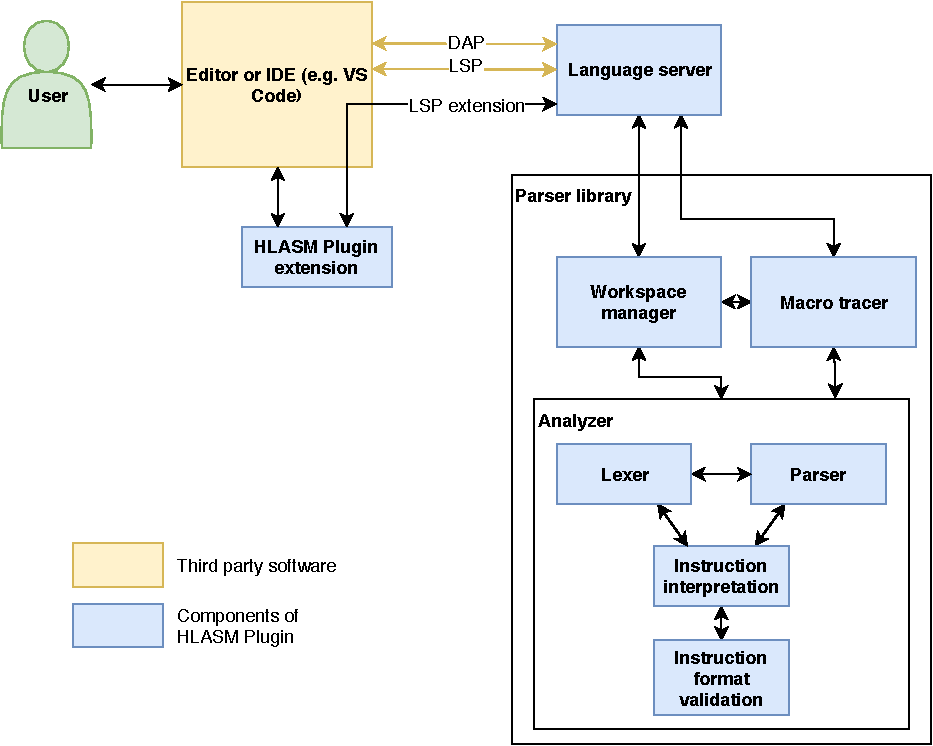
\includegraphics[width=10cm]{img/hlasm_architecture}

\end{frame}



\begin{frame}[fragile]{Preview version}

\centering
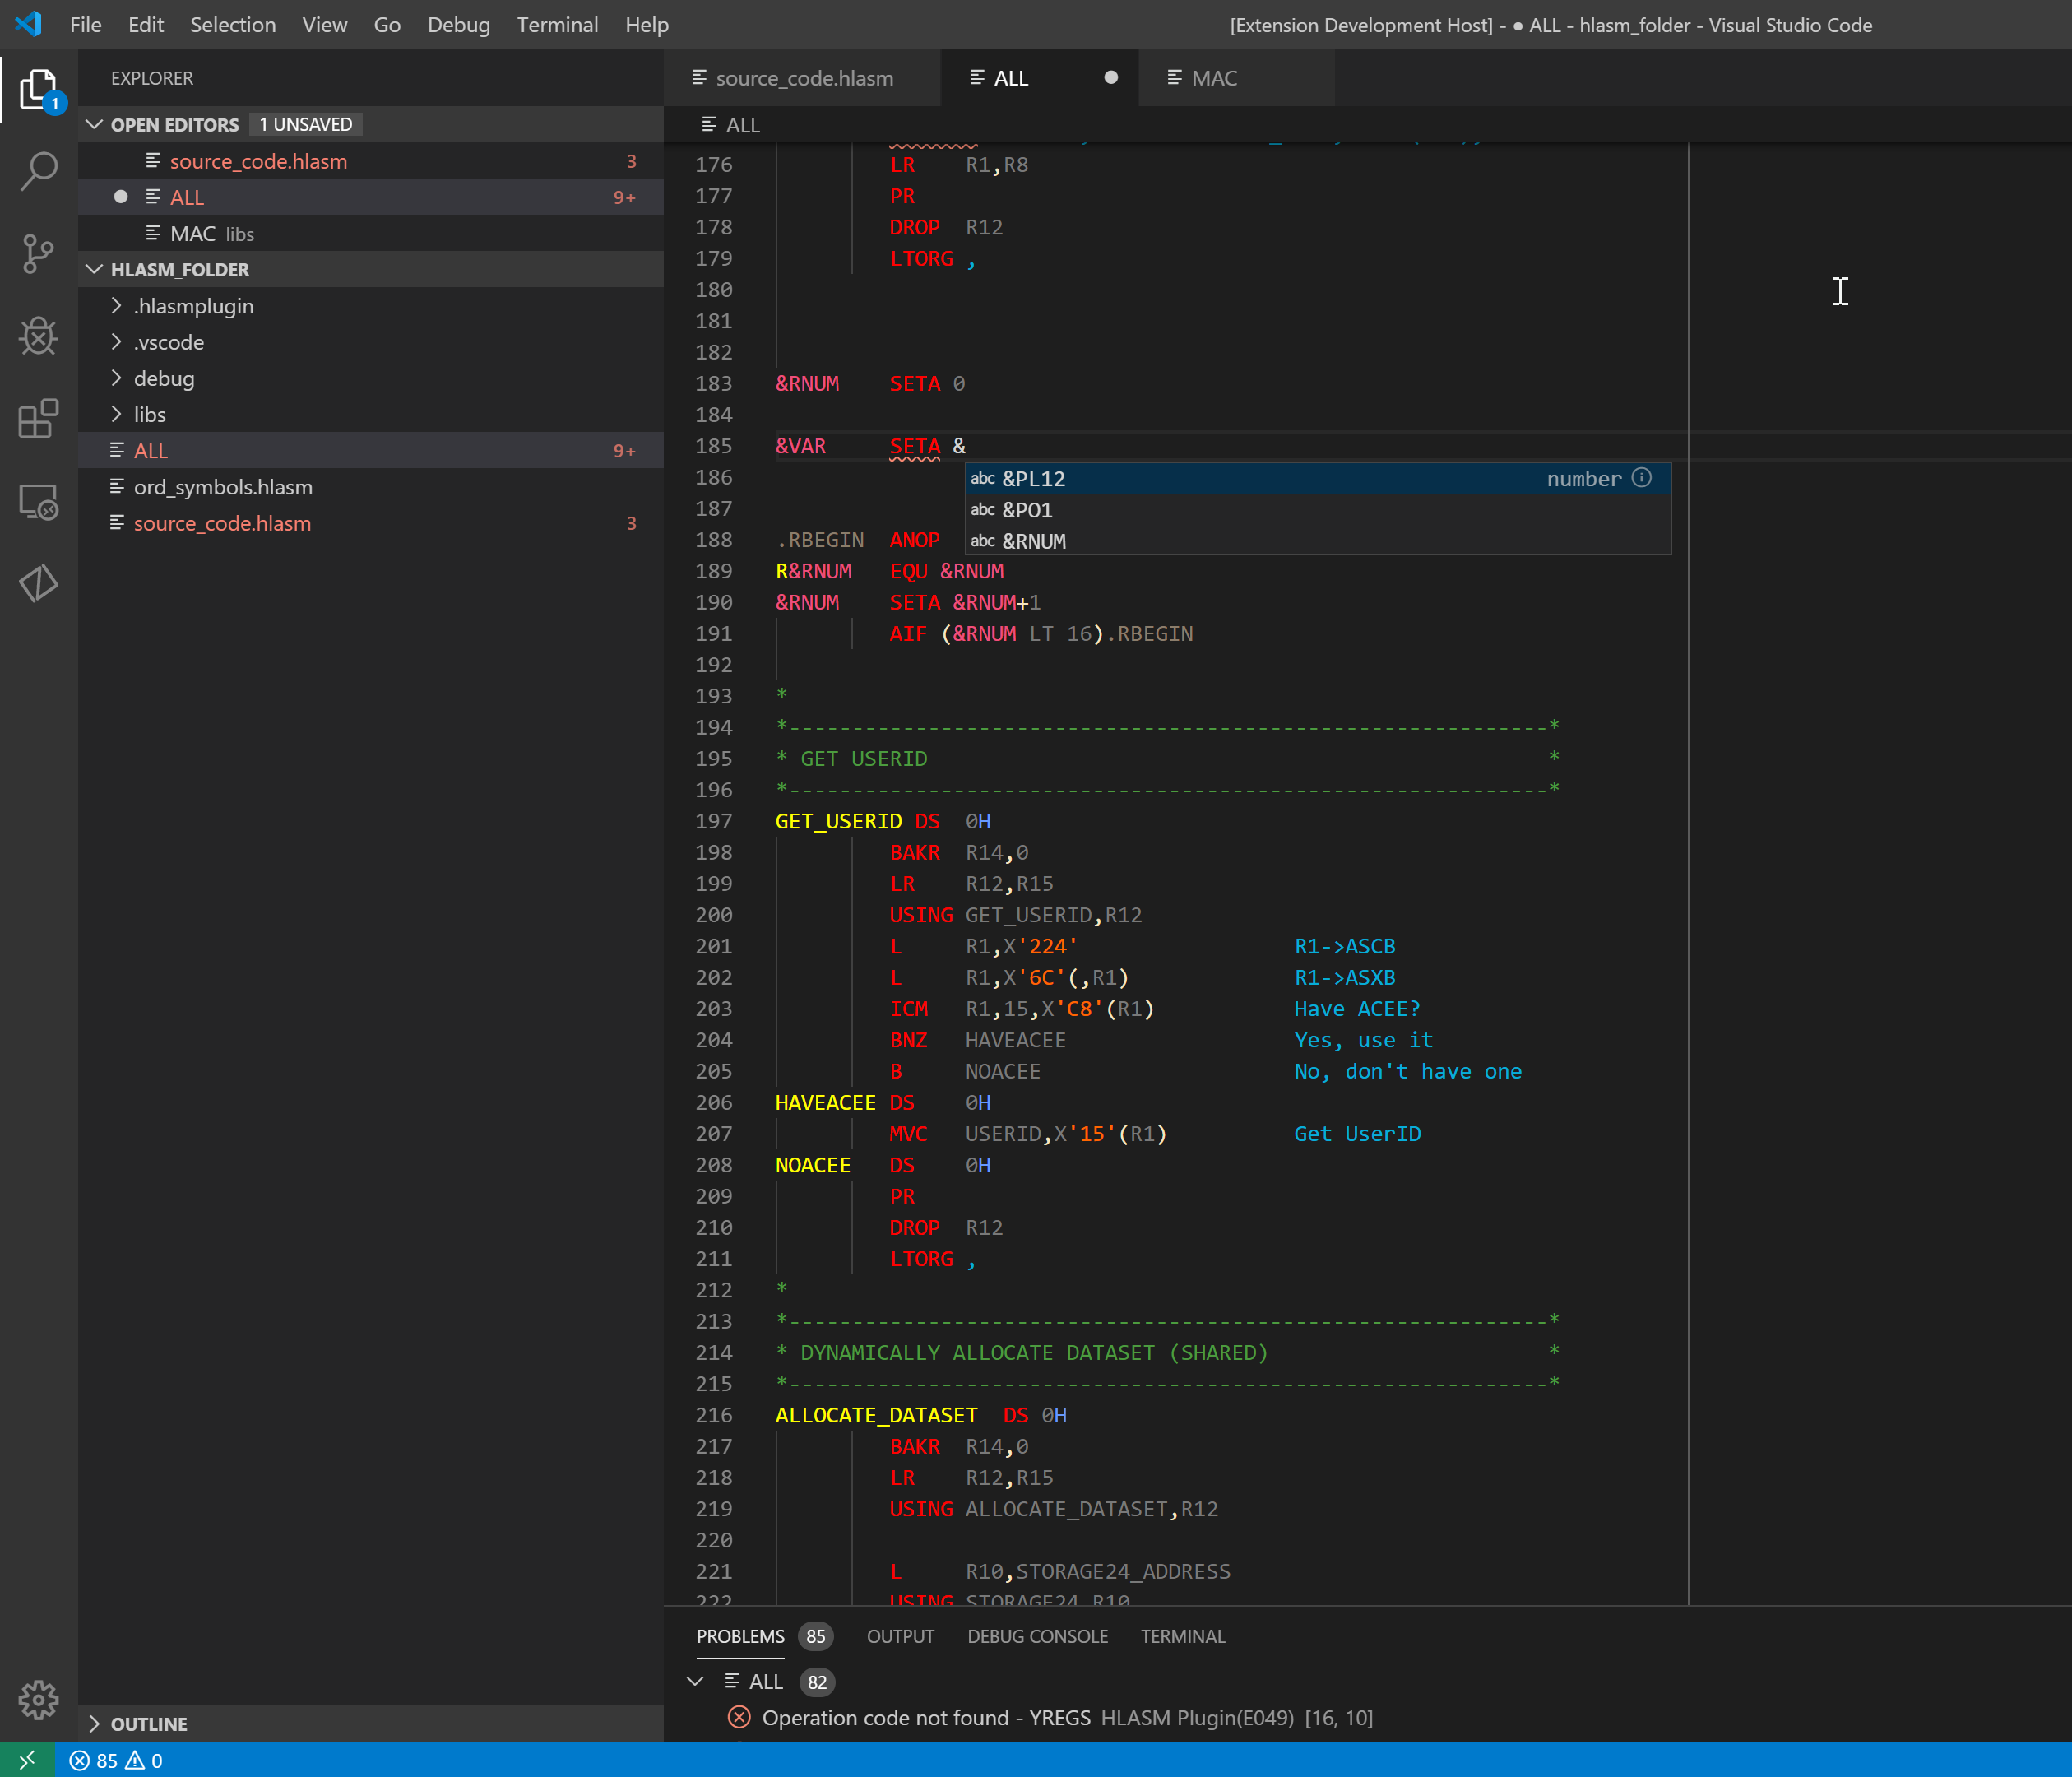
\includegraphics[width=8cm]{img/screenshot}

\small
Source code taken from \url{https://github.com/zhaimlill/EnhanceStartOnZ}

\end{frame}


\begin{frame}[fragile]{Project timeline}

\centering
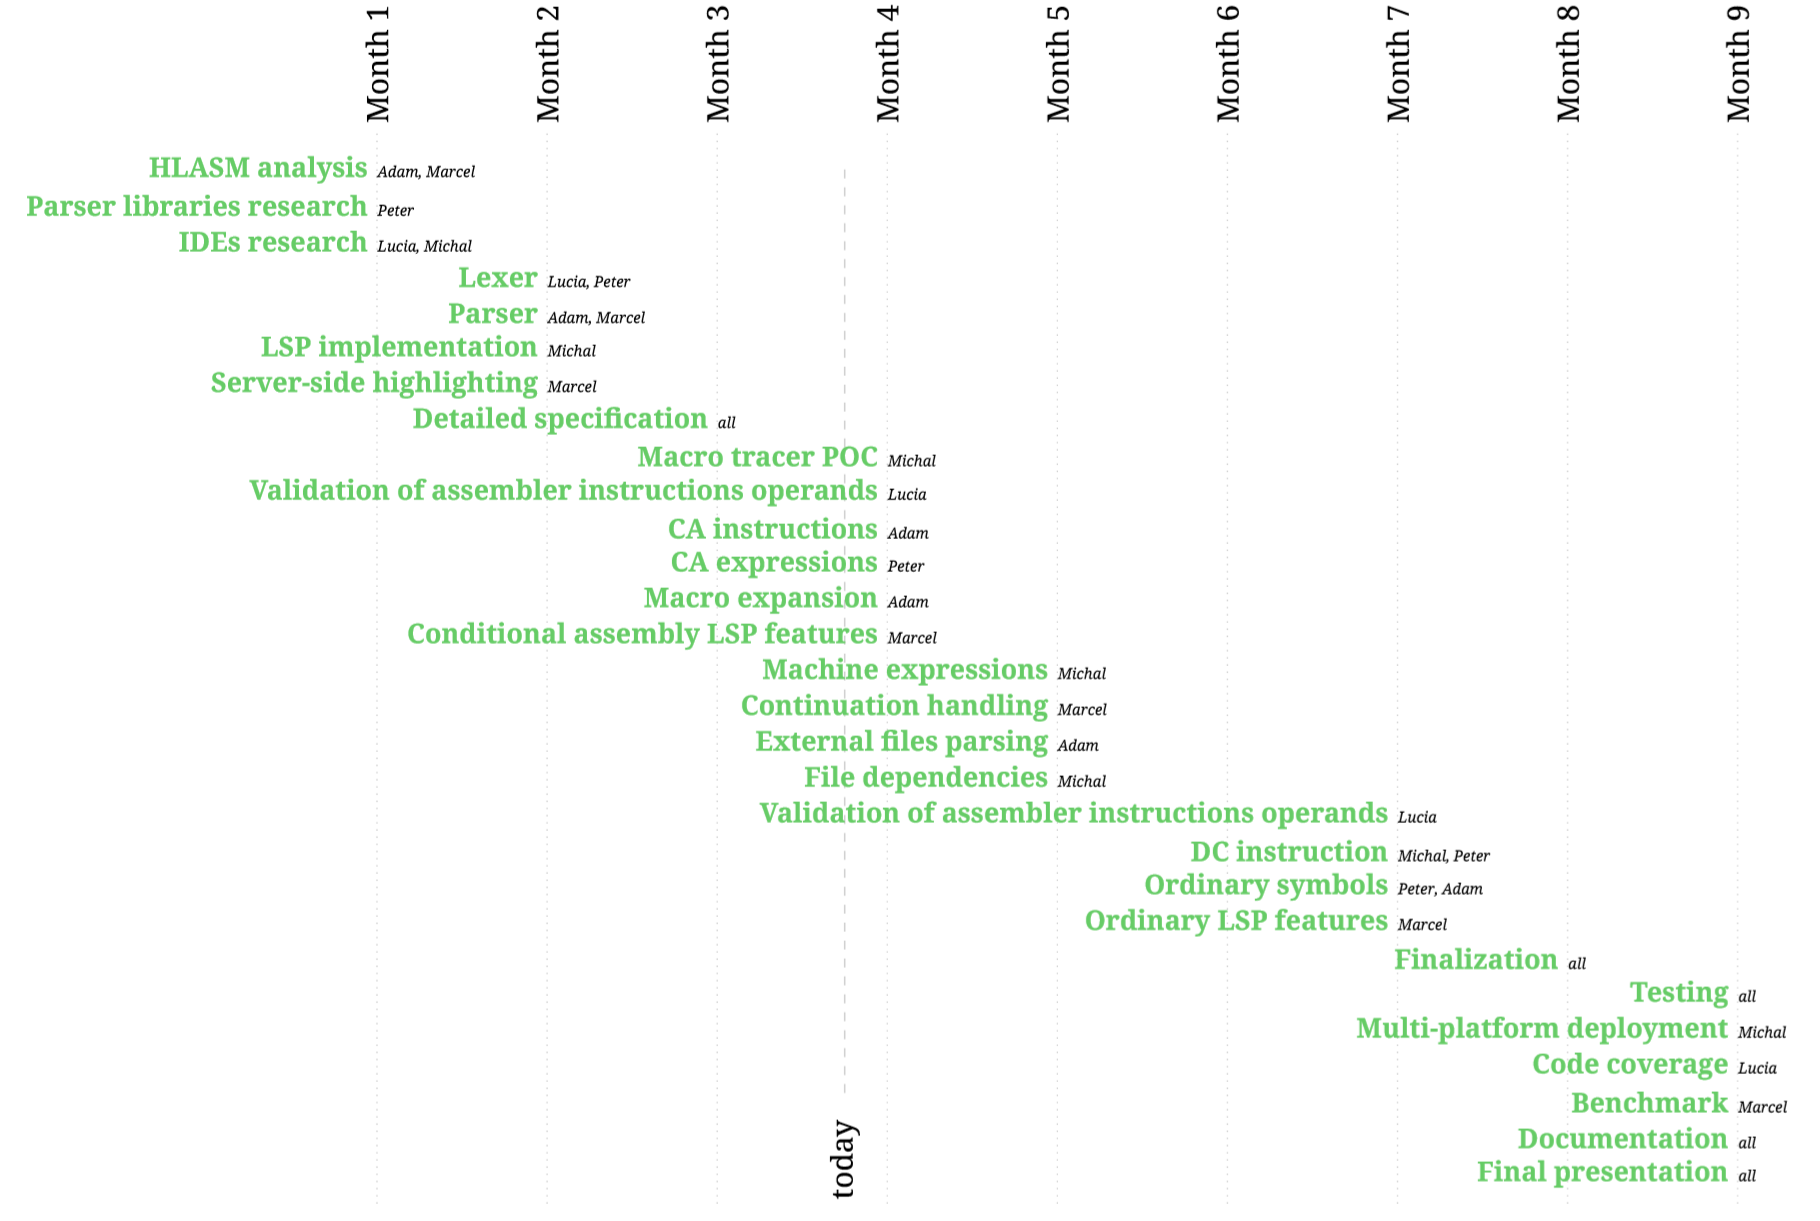
\includegraphics[width=10cm]{img/timeline}

\end{frame}


\begin{frame}[standout]
  Questions?
\end{frame}


\end{document}
